
\let\negmedspace\undefined
\let\negthickspace\undefined
\documentclass[journal]{IEEEtran}
\usepackage[a5paper, margin=10mm, onecolumn]{geometry}
%\usepackage{lmodern} % Ensure lmodern is loaded for pdflatex
\usepackage{tfrupee} % Include tfrupee package

\setlength{\headheight}{1cm} % Set the height of the header box
\setlength{\headsep}{0mm}     % Set the distance between the header box and the top of the text

\usepackage{gvv-book}
\usepackage{gvv}
\usepackage{cite}
\usepackage{amsmath,amssymb,amsfonts,amsthm}
\usepackage{algorithmic}
\usepackage{graphicx}
\usepackage{textcomp}
\usepackage{xcolor}
\usepackage{txfonts}
\usepackage{listings}
\usepackage{enumitem}
\usepackage{mathtools}
\usepackage{gensymb}
\usepackage{comment}
\usepackage[breaklinks=true]{hyperref}
\usepackage{tkz-euclide} 
\usepackage{listings}
% \usepackage{gvv}                                        
\def\inputGnumericTable{}                                 
\usepackage[latin1]{inputenc}                                
\usepackage{color}                                            
\usepackage{array}                                            
\usepackage{longtable}                                       
\usepackage{calc}                                             
\usepackage{multirow}                                         
\usepackage{hhline}                                           
\usepackage{ifthen}                                           
\usepackage{lscape}
\begin{document}

\bibliographystyle{IEEEtran}
\vspace{3cm}

\title{NCERT-10.3.3.3.3}
\author{EE24BTECH11023 - RASAGNA}

% \maketitle
% \newpage
% \bigskip
{\let\newpage\relax\maketitle}

\renewcommand{\thefigure}{\theenumi}
\renewcommand{\thetable}{\theenumi}
\setlength{\intextsep}{10pt} % Space between text and floats


\numberwithin{equation}{enumi}
\numberwithin{figure}{enumi}
\renewcommand{\thetable}{\theenumi}
\textbf{Question}\\
Form the pair of linear equations for the following problems and find their solution by
substitution method.The coach of a cricket team buys 7 bats and 6 balls for \(\text{\rupee} 3800\). Later, she buys 3 bats and 5 balls for \(\text{\rupee} 1750\). Find the cost of each bat and each ball\\
\textbf{Theoritical Solution}\\
Let the cost of each bat be \(x\) (in rupees) and the cost of each ball be \(y\) (in rupees).\\
From the problem, we can form the following equations:
\begin{align}
    7x + 6y = 3800 
\end{align}
\begin{align}
        3x + 5y = 1750 
\end{align}
Solve one equation for one variable\\
From equation \brak{0.2}
\begin{align}
    3x + 5y = 1750 
\end{align}
\begin{align}
        3x = 1750 - 5y
\end{align}
\begin{align}
        x = \frac{1750 - 5y}{3} 
\end{align}
Substitute \(x\) into equation \brak{0.1}
\begin{align}
    7x + 6y = 3800
\end{align}
\begin{align}
        7 \left( \frac{1750 - 5y}{3} \right) + 6y= 3800 
\end{align}
\begin{align}
        \frac{7(1750 - 5y)}{3} + 6y= 3800 
\end{align}
\begin{align}
        \frac{12250 - 35y}{3} + 6y = 3800
\end{align}
Simplifying further,
\begin{align}
    12250 - 35y + 18y = 11400 
\end{align}
\begin{align}
    -17y = -850    
\end{align}
\begin{align}
       \therefore y = 50
\end{align}
Now,Substitute \(y = 50\) into equation \brak{0.5};
\begin{align}
    x = \frac{1750 - 5(50)}{3} 
\end{align}
\begin{align}
        x = \frac{1500}{3} 
\end{align}
\begin{align}
    \therefore x = 500
\end{align}
\textbf{Computational Solution}
\section*{LU Factorization Solution}
Given a matrix $A$ of size $n \times n$, LU decomposition is performed row by row and column by column. The update equations are as follows:
We Start by initializing $L$ as the identity matrix $L = I$ and $U$ as a copy of $A$.
For each column $j \geq k$, the entries of $U$ in the $k$-th row are updated as:
\begin{align}
U_{k,j} = A_{k,j} - \sum_{m=1}^{k-1} L_{k,m} \cdot U_{m,j}, \quad \forall \, j \geq k 
\end{align}
For each row $i > k$, the entries of $L$ in the $k$-th column are updated as:
\begin{align}
L_{i,k} = \frac{1}{U_{k,k}} \left( A_{i,k} - \sum_{m=1}^{k-1} L_{i,m} \cdot U_{m,k} \right), \quad \forall \, i > k 
\end{align}

We are solving the following system of linear equations:
\begin{align}
7x + 6y = 3800
\end{align}
\begin{align}
3x + 5y = 1750
\end{align}
In matrix form:
\[
\begin{bmatrix}
7 & 6 \\
3 & 5
\end{bmatrix}
\begin{bmatrix}
x \\
y
\end{bmatrix}
=
\begin{bmatrix}
3800 \\
1750
\end{bmatrix}
\]
Where,
\[
A = 
\begin{bmatrix}
7 & 6 \\
3 & 5
\end{bmatrix}, \quad
\mathbf{x} = 
\begin{bmatrix}
x \\
y
\end{bmatrix}, \quad
\mathbf{b} = 
\begin{bmatrix}
3800 \\
1750
\end{bmatrix}
\]
The LU decomposition expresses \(A\) as:
\begin{align}
    A = L \cdot U
\end{align}
Where,
\begin{align}
    L = 
\begin{bmatrix}
1 & 0 \\
l_{21} & 1
\end{bmatrix}, \quad
U = 
\begin{bmatrix}
u_{11} & u_{12} \\
0 & u_{22}
\end{bmatrix}
\end{align}
Compute \(L\) and \(U\)
\begin{align}
u_{11} &= 7, \quad u_{12} = 6 \\
l_{21} &= \frac{A[2,1]}{u_{11}} = \frac{3}{7} \\
u_{22} &= A[2,2] - l_{21} \cdot u_{12} = 5 - \frac{3}{7} \cdot 6 = \frac{17}{7}
\end{align}
Thus:
\[
L = 
\begin{bmatrix}
1 & 0 \\
\frac{3}{7} & 1
\end{bmatrix}, \quad
U = 
\begin{bmatrix}
7 & 6 \\
0 & \frac{17}{7}
\end{bmatrix}
\]
Solve \(L \cdot \mathbf{y} = \mathbf{b}\)
\begin{align}
\begin{bmatrix}
1 & 0 \\
\frac{3}{7} & 1
\end{bmatrix}
\begin{bmatrix}
y_1 \\
y_2
\end{bmatrix}
&=
\begin{bmatrix}
3800 \\
1750
\end{bmatrix}
\end{align}
Solving,\\
\begin{align}
\implies y_1 &= 3800
\end{align}
\begin{align}
\implies \frac{3}{7} \cdot 3800 + y_2 &= 1750 \\
y_2 &= 1750 - \frac{3}{7} \cdot 3800 \\
y_2 &= 1750 - \frac{11400}{7} = \frac{850}{7}
\end{align}
Thus,
\begin{align}
    \mathbf{y} = 
\begin{bmatrix}
3800 \\
\frac{850}{7}
\end{bmatrix}
\end{align}
Solve \(U \cdot \mathbf{x} = \mathbf{y}\)
\begin{align}
\begin{bmatrix}
7 & 6 \\
0 & \frac{17}{7}
\end{bmatrix}
\begin{bmatrix}
x \\
y
\end{bmatrix}
&=
\begin{bmatrix}
3800 \\
\frac{850}{7}
\end{bmatrix}
\end{align}
Solving,\\
\begin{align}
\implies \frac{17}{7} \cdot y &= \frac{850}{7} \\
y &={\frac{850}{7}} \cdot \frac{7}{17} = 50
\end{align}
\begin{align}
\implies 7x + 6y &= 3800 \\
7x + 6 \cdot 50 &= 3800 \\
7x &= 3800 - 300 = 3500 \\
x &= \frac{3500}{7} = 500
\end{align}
Final computed Solution \\
Cost of one bat (x): 500.00\\
Cost of one ball (y): 50.00\\
\begin{center}
    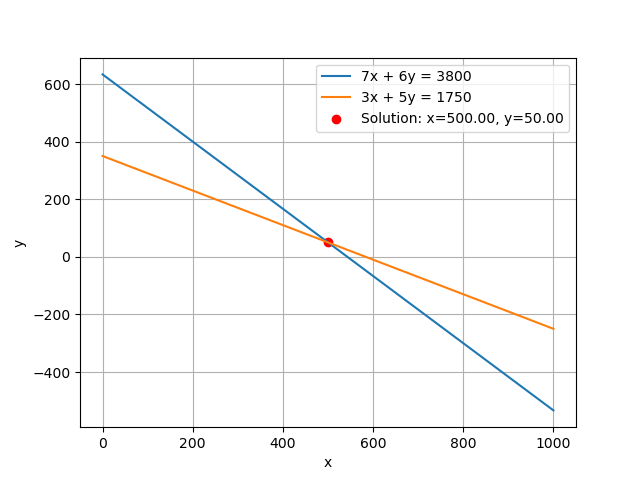
\includegraphics[width=0.75\columnwidth]{figs/fig33.png}
\end{center}

\end{document}